\documentclass[11]{article}

\usepackage[backend=bibtex]{biblatex}
\bibliography{references}

\usepackage{graphicx}

\begin{document}

\section{Review : Contour Matching Techniques}

\subsection{Motivation}
In optimising our tool positional search, we can determine the regions of contact that are more likely to be good fit for the active and passive object interaction. This follows the ideas proposed by \cite{battaglia2013}, in that humans build mental models of objects to allow inference over  the physical world. Human subjects would therefore have understanding of the geometric constraints of the physical world and of the forces generated by their actions.

Interaction with a high likelihood for success would have to satisfy two criteria: 
\begin{enumerate}
\item \textbf{Geometric constraints} of the two objects must be met ( i.e. the shapes of the two objects should adequately fit )
\item \textbf{Contact forces} generated must correspond to the intention of the actions executed (i.e. for a lifting action, the human subject would focus on points of interaction that would permit vertical forces to be applied)
\end{enumerate}

The total space of possible solutions can be reduced by these criteria without explicit simulation (akin mental simulations\cite{osiurak2014}). The physics engine would later verify the potential of different solutions. 

\subsection{Geometric Constraints}
The geometries of the tool and object must be compatible. In other words, either the active or passive object's geometry must fit within the gaps and edges of its counterpart. Tighter fits, offer better transfer of energy and control over the movement of the passive object. A better fit would therefore require less manipulation effort. In the paradigm of 4CT \cite{osiurak2014}, the effort constraint may explain user's preference for one geometric solution over another.

It is not necessary for the whole geometry of objects to fit. It is sufficient for the tool to have the necessary parts acting as affordance and functional basis (end effector\cite{zhu2015}). If the functional part matches the gaps of the passive object, then the configuration is likely to achieve the desired effect. 

\subsubsection{Shape Description and Matching}

We consider techniques of shape similarity in matching object parts. Shape analysis techniques have traditionally been engaged in image processing and robot vision for detecting and tracking objects of similar features. The last two decades have provided many approaches for this type of problem \cite{loncaric1998,zhang2004,veltkamp2001,robert2012}. Fundamentally, the callenge lies in detecting similarit even as objects undergo geometric transformations (i.e. rotation,translation,scalling and shearing).     

Zhang\cite{zhang2004} et al. classify shape similarity into contour-based and region-based techniques. These are further divided into structural and global approaches. A comprehensive list and structure can be found in fig. \ref{fig:shape_similarity}.

\begin{figure}[h]
  \centering
  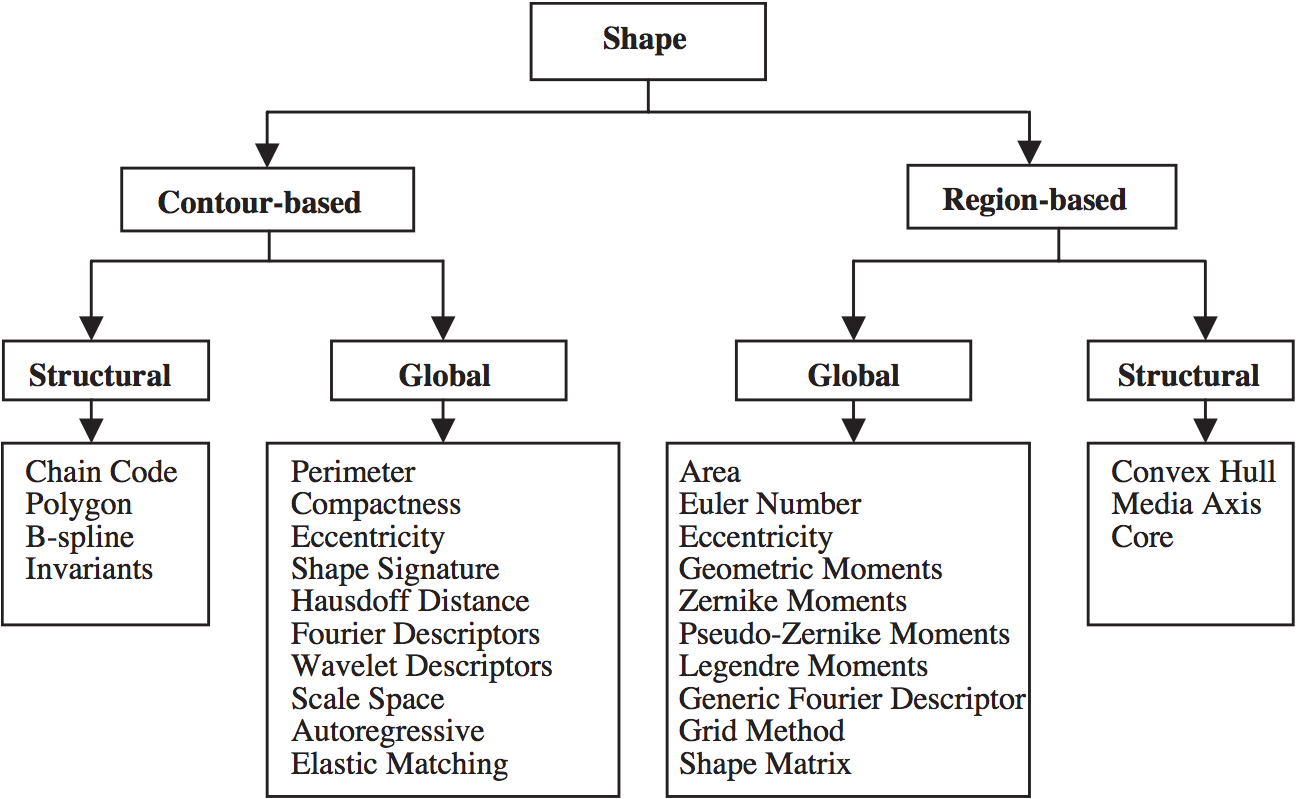
\includegraphics[width=1\textwidth]{./figures/similarity_techniques.png}
  \caption{Classification of shape similarity techniques (reprinted from \cite{zhang2004})}
  \label{fig:shape_similarity}
\end{figure}  

Contour techniques asses shape similarity by extracting features from the edge of detected objects. In comparison, region techniques work by assessing surface level information such as: colour features, gradient changes and surface medial. Techniques from both approaches have justification in human perception \cite{chatbri2016}. Nontheless, our use case excludes most reagion-based approaches. Tool parts must corespond to shape gaps. It is hard to consider gaps as having the surface information needed for region-based matching.

In structural appraches, shapes are considered as composed out of primitives. In the case of contour techniques, primitives are segments on the boundry of an object. The organisation of primitives can be linear (feature vector\cite{zhang2004}) or hierarchical (tree like structures\cite{zhu2015}). Two objects are considered similiar when they have the same primitive structures (or features). In comparison, global approaches make use of shapes as a whole when assesing similarity. 

Both structural and global approaches have justification in human perception \cite{zhang2004}. Human subjects show a preference for features even when other shape descriptors are available \cite{chatbri2016}. At the same time, global shape perception seems to preceed local feature detection\cite{navon1977}. 

Matching human behaviour requires more insight into human visual perception. Loncaric\cite{loncaric1998} describes some theories of human visual perception with interest in image processing. In a tool use scenario, more interest should be given to theories describing perception as volumetric, such as through the use of generalised cylinders (geons\cite{dickinson2014}). Such insight may however be of use in future work.    

\printbibliography
\end{document}

